% !TeX spellcheck = en_US 
\subsection{Results}
In order to simulate interlocking structures with a range of design parameters we automatically generate INP files in Abaqus CAE (2020) using a script.
Solving an INP file gives us the force-displacement graph, from which we can determine the ultimate tensile strength of a particular design.
In order to simulate accurately we used the stress-strain curves from tensile tests on the base materials printed flat on the \revise{build plate}{build platform} as the plasticity in tabular form.
The simulations were performed in the Abaqus/Explicit solver where the Dynamic, Explicit procedure step was used with a mass scaling factor of $10^7$,
using geometric nonlinearity and general contact (explicit) to disregard friction for simplicity.

The repeating nature of the interlocking patterns was captured by modelling half of the unit cell and applying symmetry constraints to the sides, top and bottom.
The model was meshed using C3D8R hexahedral elements of $\pm\SI{75}{\micro\meter}$.

A grid search was used to measure the influence on the ultimate strength along each of the design variables $\wb,\va, \hc$, along with the total length $L$.
The search space was therefore 4D and 2D for the straight and diagonal ITIM model respectively.
In order to estimate the optimum we fit a smooth response surface to these data points using a radial basis function (RBF) network\cite{Dinh2002},
with a smoothness of $\lambda=1$.


\subsubsection{Straight ITIM variant}
In order to prevent stress concentrations and adhere to manufacturing accuracy, the vertical edges of the straight ITIM variant were rounded with $r=\SI{0.15}{\milli\meter}$;
see \cref{interlocking:fig:sim_straight_model}.
%We performed two rounds of hypersurface fitting on grid search; the second round was on a zoomed in region and with elements of $\pm\SI{50}{\micro\meter}$.

Newton's method was used to determine the optimum, starting from the best sampled point.
This step only considered the dimensions $\wb$ and $\va$, because $\lmax$ is given and $\hf$ has to be an integer multiple of $\hmin$.
%\footnote{It's unlikely the optimum of the fitted hypersurface would be on a different integer multiple of $\hmin$.}
The resulting hypersurfaces are visualized in \cref{interlocking:fig:simulation_results_straight}.
The obtained optima are shown in \cref{interlocking:tab:sim_straight_optima}.

We compare these results to our analytical model by adjusting the analytical model to capture the inaccurate Z strength used in the simulations:
$\sigmafailz{m} := \sigmafail{m}$.
See \cref{interlocking:fig:ana_sim_accuracy_straight}.
We then observe that our analytical model on average predicts only \SI{7.8}{\percent} higher ultimate strength values than then the FEM simulations, with a standard deviation of \SI{16.2}{\percent}.

\begin{figure}
	\centering
	\setlength{\figheight}{.32\columnwidth}
	\begin{subfigure}[B]{.6\columnwidth}
		\centering
		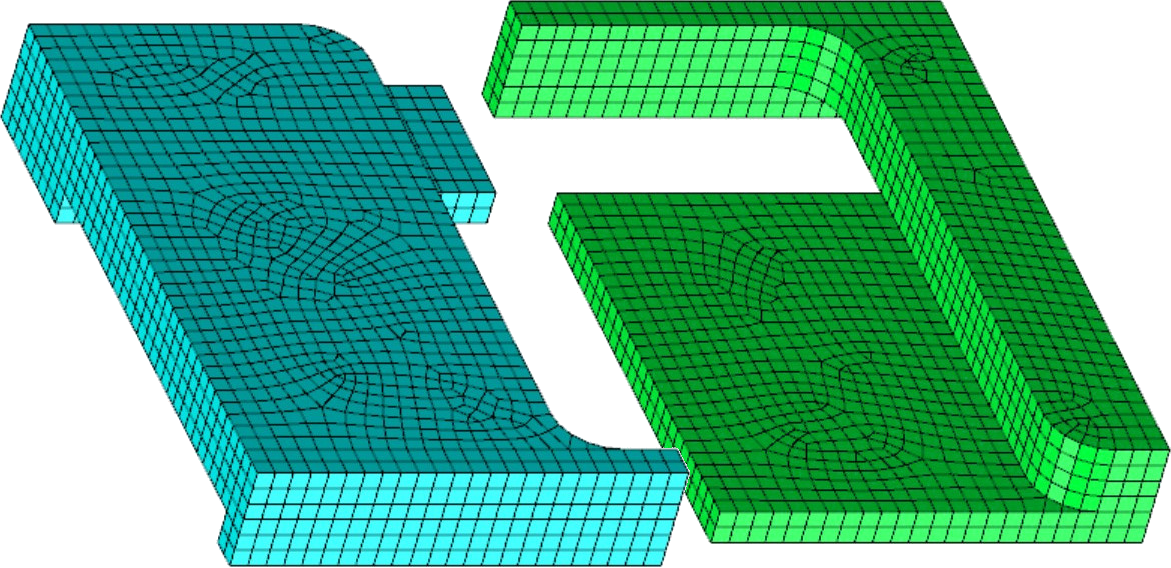
\includegraphics[height=\figheight]{sources-simulation-mesh-straight.png}
		\caption{Straight ITIM}
	\end{subfigure}
\hspace{-.5cm}
	\begin{subfigure}[B]{.39\columnwidth}
		\centering
		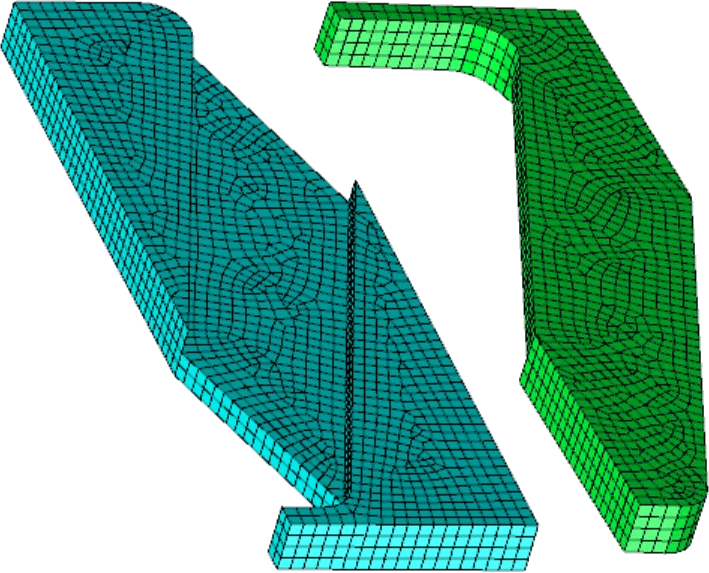
\includegraphics[height=\figheight]{sources-simulation-mesh-diagonal.png}
		\caption{Diagonal ITIM}
	\end{subfigure}
	\caption{Example simulation meshes.
		The mesh of the diagonal ITIM variant is half a unit cell covering only one of the two diagonal fingers.
		Because of the rounded corners an axis aligned meshing was impossible, leading to singularities in the mesh.}
	\label{interlocking:fig:sim_straight_model}
\end{figure}



\begin{figure*}
	\centering
	\setlength{\figheight}{.25\textwidth}
	\begin{subfigure}[B]{.48\columnwidth}
		\centering
		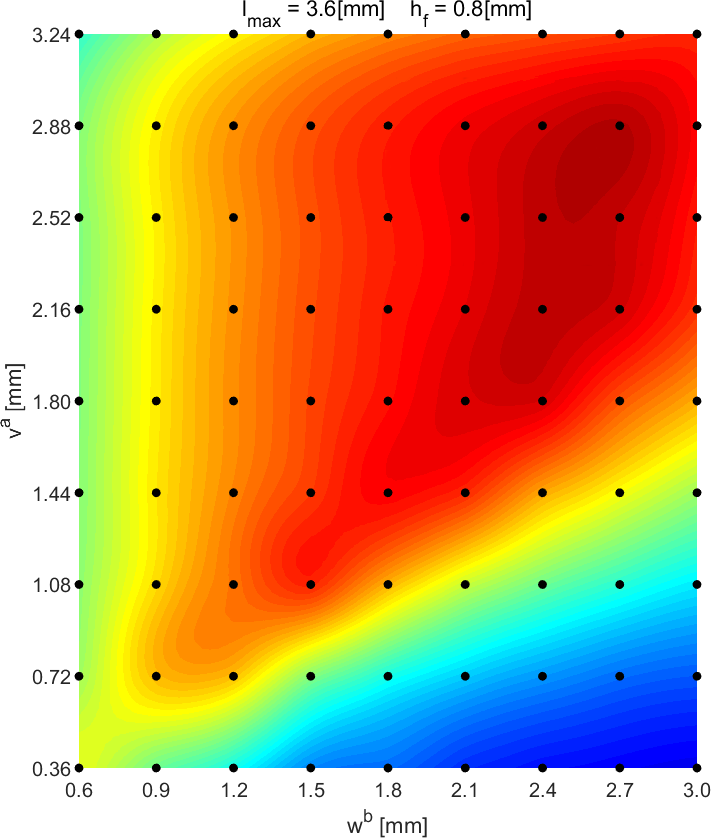
\includegraphics[height=\figheight]{sources-simulation-r1-lmax3.6.png}
		\caption{$\lmax=\SI{3.6}{\milli\meter}; \hf=\SI{0.8}{\milli\meter}$}
	\end{subfigure}
	\begin{subfigure}[B]{.48\columnwidth}
		\centering
		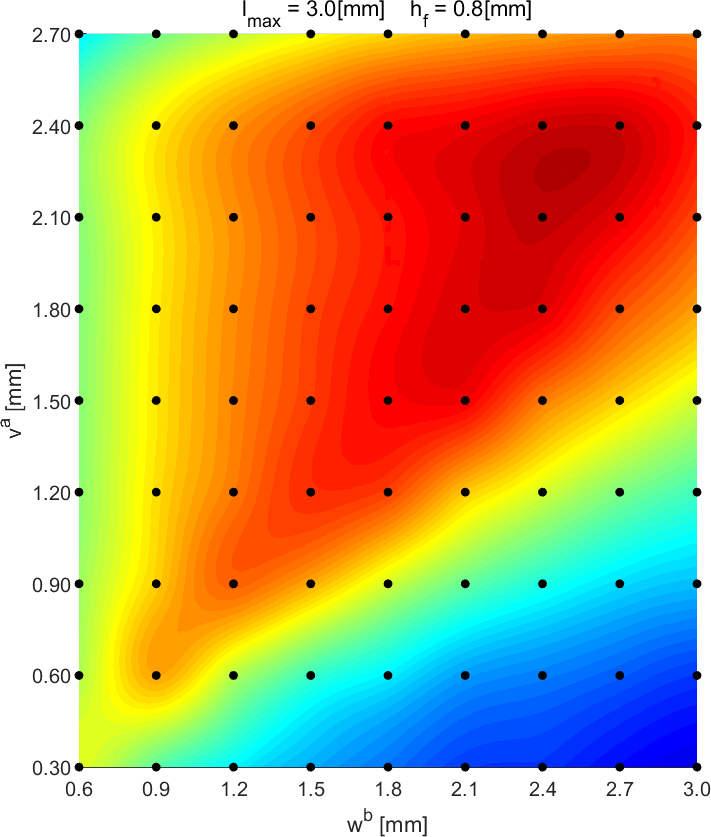
\includegraphics[height=\figheight]{sources-simulation-r1-lmax3.0.png}
		\caption{$\lmax=\SI{3.0}{\milli\meter}; \hf=\SI{0.8}{\milli\meter}$}
	\end{subfigure}
	\begin{subfigure}[B]{.48\columnwidth}
		\centering
		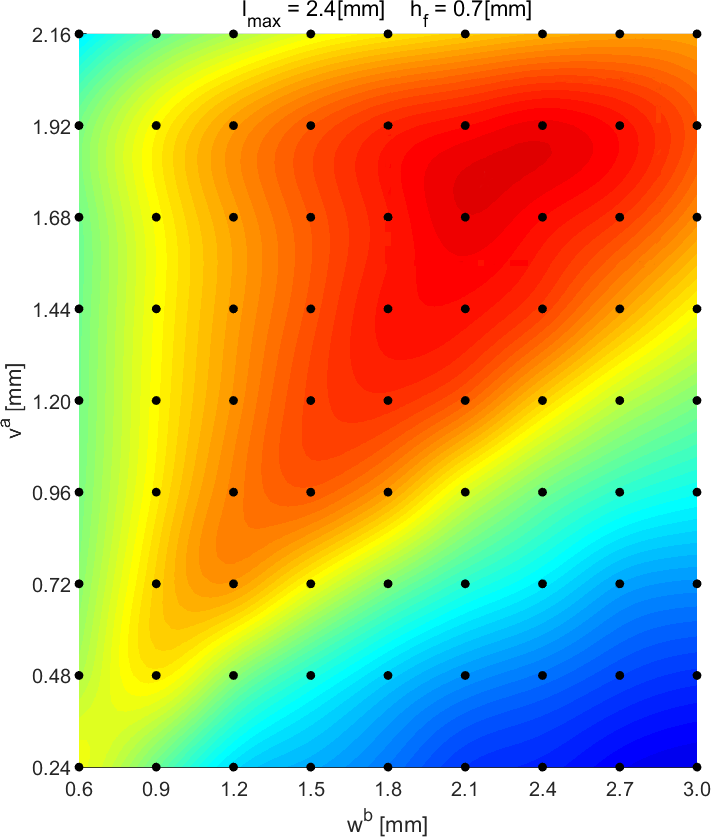
\includegraphics[height=\figheight]{sources-simulation-r1-lmax2.4.png}
		\caption{$\lmax=\SI{2.4}{\milli\meter}; \hf=\SI{0.7}{\milli\meter}$}
	\end{subfigure}
	\begin{subfigure}[B]{.52\columnwidth}
		\centering
		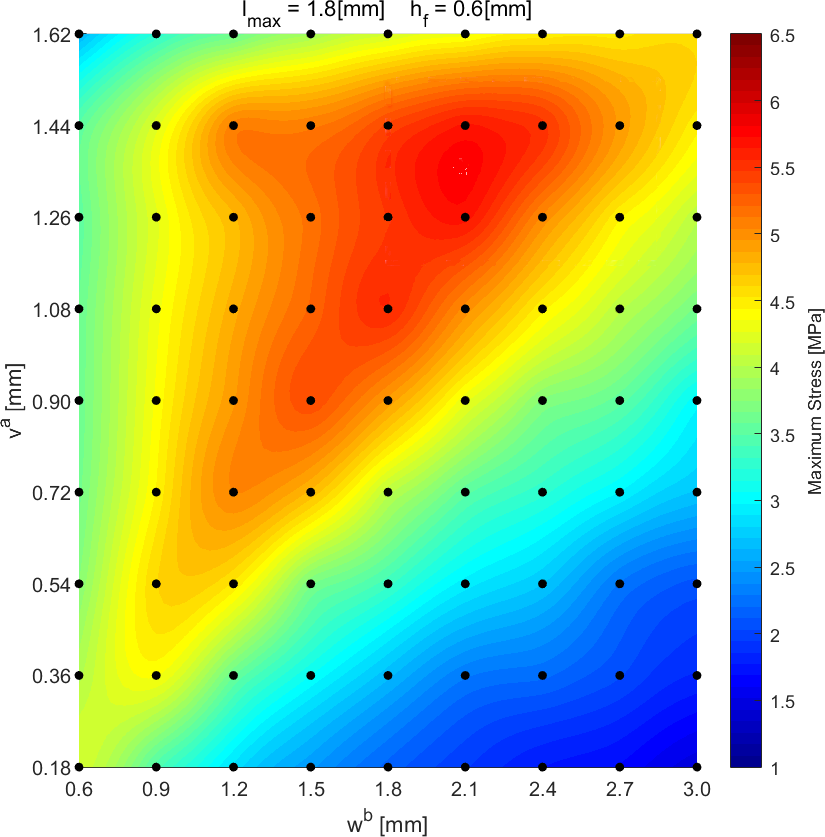
\includegraphics[height=\figheight]{sources-simulation-r1-lmax1.8.png}
		\caption{$\lmax=\SI{1.8}{\milli\meter}; \hf=\SI{0.6}{\milli\meter}$}
	\end{subfigure}
	\caption{2D slices of the 4D simulation results and fitted RBF hypersurface for the straight ITIM variant. Sampled data points in black.}
	\label{interlocking:fig:simulation_results_straight}
\end{figure*}


\begin{figure*}
	\centering
	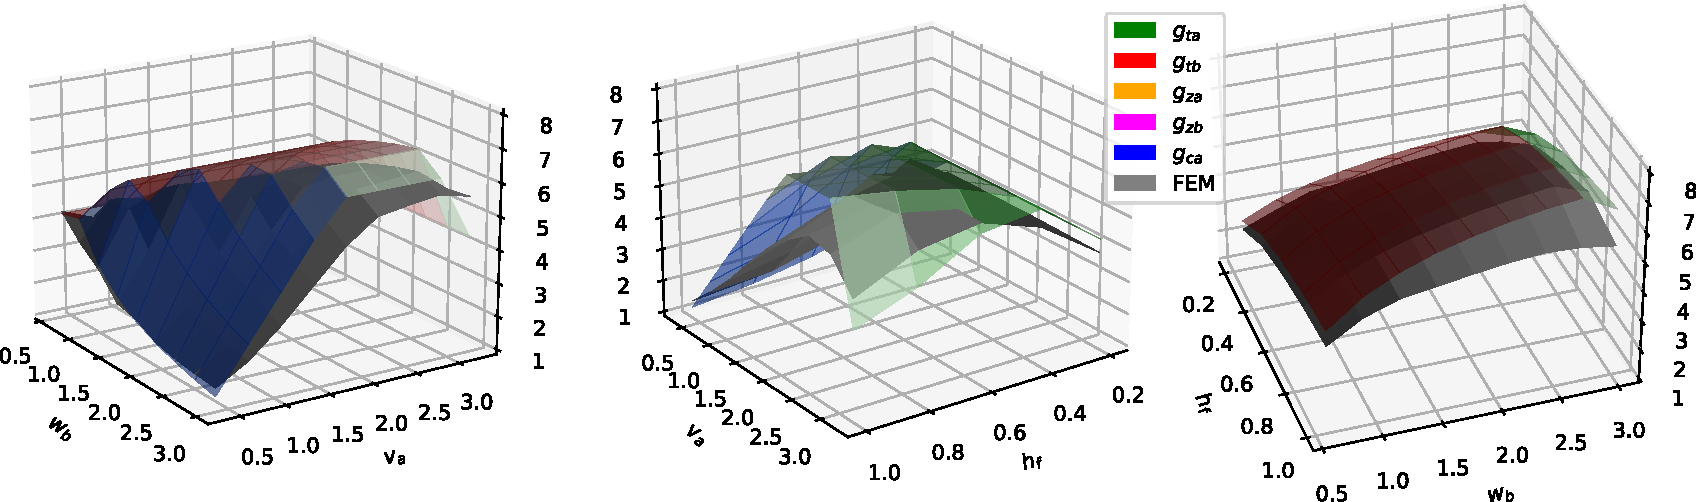
\includegraphics[width=.8\textwidth]{sources-simulation-model_accuracy.pdf}
	\caption{Ultimate strength according to the analytical models and the simulation results for the straight variant of the ITIM lattice.
		The analytical models follow roughly the same shape and same height as the simulation results. 
		The response on three 2D slices of the 3D design space are shown, from left to right at $\hf=0.8$, $\wb=2.7$ and at $\va=2.88$.
	}
	\label{interlocking:fig:ana_sim_accuracy_straight}
\end{figure*}



\begin{table}
	\caption{Optimal designs according to the hypersurface fitted to the FEM simulations for the straight ITIM variant and for the diagonal ITIM variant.}
	\label{interlocking:tab:sim_straight_optima}
	\begin{tabular}{ll|llll}
		&$\lmax$ (\si{\milli\meter})             & 3.6 & 3.0 & 2.4 & 1.8 \\
		\hline
		\multirow{4}{*}{\rotatebox[origin=c]{90}{straight}}
		&$\sigma_\text{max}$ (\si{\mega\pascal}) & \bf 6.17 & \bf 6.12 & \bf 5.89 & \bf 5.59 \\
		&$\hf$ (\si{\milli\meter})               & 0.8 & 0.8 & 0.7 & 0.6 \\
		&$\wb$ (\si{\milli\meter})               & 2.58 & 2.42 & 2.17 & 2.05 \\
		&$\va$ (\si{\milli\meter})               & 2.67 & 2.23 & 1.78 & 1.35 \\
		\hline
		\multirow{2}{*}{\rotatebox[origin=c]{90}{diag}}
		&$\sigma_\text{max}$ (\si{\mega\pascal}) & \bf 6.30 & \bf 6.37 & \bf 5.86 & \bf 4.69 \\
		&$\wb$ (\si{\milli\meter})               & 1.21 & 1.19 & 1.18 & 1.04 \\
		\end
		{tabular}
\iffalse
	\begin{tabular}{l|llllllll}
		Round & 1 & 2 & 1 & 2 & 1 & 2 & 1 & 2 \\
		\hline
		$\lmax$ (\si{\milli\meter}) & 3.6 & 3.6 & 3.0 & 3.0 & 2.4 & 2.4 & 1.8 & 1.8\\
		$\hf$ (\si{\milli\meter}) & 0.8 & 0.8 & 0.8 & 0.8 & 0.7 & 0.7 & 0.6 & 0.6 \\
		$\wb$ (\si{\milli\meter}) & 2.58 & 2.54 & 2.42 & 2.35 & 2.18 & 2.22 & 2.05 & 2.01\\
		$\va$ (\si{\milli\meter}) & 2.67 & 2.82 & 2.23 & 2.27 & 1.78 & 1.84 & 1.35 & 1.36 \\
		$\sigma_\text{max}$ (\si{\mega\pascal}) & 6.17 & 6.11 & 6.12 & 6.03 & 5.89 & 5.81 & 5.59 & 5.53
	\end{tabular}
\fi
\end{table}





\subsubsection{Diagonal ITIM variant}
Modelling the diagonal ITIM variant in Abaqus can be quite cumbersome, since it does not natively support periodic boundary constraints.
Whereas this problem can be overcame in the straight ITIM variant because it is symmetric,
the diagonal variant is only \emph{rotationally} symmetric.
While a symmetry constraint can be used on the top and bottom, the two sides of the design are mirror images of each other, but also flipped vertically.

However, since the height of the beams is relatively low compared to their width we have observed that the stresses and strains are quite similar in the top and bottom.
If we model half of the diagonal ITIM cell by cutting it vertically and apply symmetry constraints to the sides,
the induced error is only $\pm \SI{10}{\percent}$ compared to simulating an interface consisting of two whole cells.
% small discontinuities



\begin{figure}
	\centering
	\begin{subfigure}[B]{.49\columnwidth}
		\centering	
		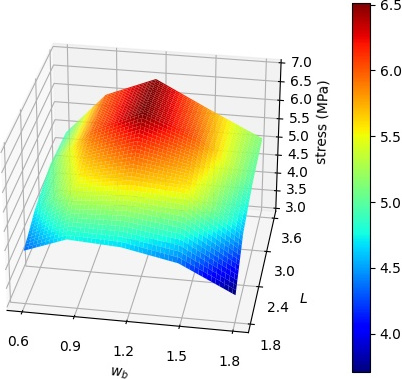
\includegraphics{sources-simulation-diagonal_sim_response.jpg}
		\caption{Simulation results.}
		\label{interlocking:fig:sim_diagonal_model}
	\end{subfigure}
	\begin{subfigure}[B]{.49\columnwidth}
		\centering
		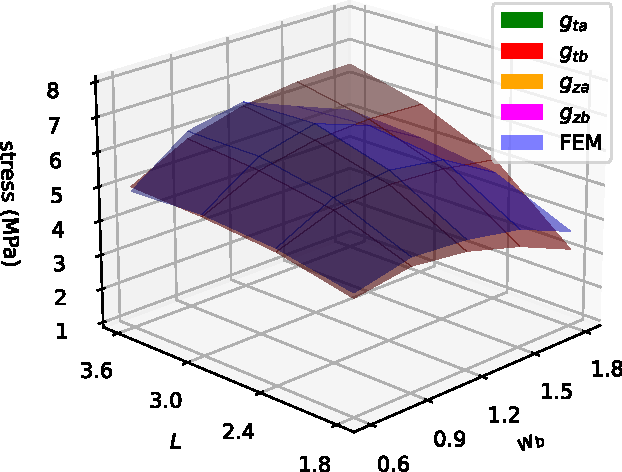
\includegraphics{sources-simulation-model_accuracy_diagonal.pdf}
		\caption{The analytical model follows the simulation results rather well at lower $\wb$ values.}
		\label{interlocking:fig:ana_sim_accuracy_diagonal}
	\end{subfigure}
	\caption{Simulation results for diagonal ITIM variant using linear interpolation between the simulation results.}
\end{figure}


The results of these simulations are shows in \cref{interlocking:fig:sim_diagonal_model}.
%The predictions from the analytical model can directly be compared to the simulation results, because the constraints on Z shear are not active. < What do I mean here?!
We compare the simulations against our analytical model in \cref{interlocking:fig:ana_sim_accuracy_diagonal}.
The analytical model predicts only 0.4\% lower ultimate strength values on average with a standard deviation of 10\%.

%optimal designs table








